\documentclass[xcolor=pdftex,romanian,colorlinks]{beamer}

\usepackage[export]{adjustbox}
\usepackage{../tslides}
\usepackage[all]{xy}
\usepackage{pgfplots}
\usepackage{flowchart}
\usepackage{comment}
\usetikzlibrary{arrows,positioning,calc}
\lstset{language=Haskell}
\lstset{escapeinside={(*@}{@*)}}

\AtBeginSection[]{
  \begin{frame}
  \vfill
  \centering
  \begin{beamercolorbox}[sep=8pt,center,shadow=true,rounded=true]{title}
    \usebeamerfont{title}\insertsectionhead\par%
  \end{beamercolorbox}
  \vfill
  \end{frame}
}


\title[PD---Monade]{Programare declarativă\thanks{bazat pe cursul \emph{Informatics 1: Functional Programming} de la \emph{University of Edinburgh}}}

\subtitle{De la functori la monade}

\begin{document}
\begin{frame}
  \titlepage
\end{frame}

\section{Functori}

\subsection{Matematică}

\begin{frame}{Categorii}

\begin{block}{Intuiție}
O categorie este dată de \structure{obiecte} și \alert{săgeți} între ele
\end{block}
\begin{block}{Exemple}
\begin{description}
\item[$\mathbb Set$:] \structure{mulțimi} și \alert{funcții}
\item[$\mathbb Poset$:] \structure{Mulțimi parțial ordonate} și \alert{funcții monotone}
\item[$\mathbb Mon$:] \structure{Monoizi} și \alert{morfisme de monoizi}
\item[$\mathbb Top$:] \structure{spații topologice} și \alert{morfisme de spații topologice}
\item[$\mathbb Hask$:] \structure{tipuri} și \alert{funcții} în Haskell
\end{description}
\end{block}
\end{frame}

\begin{frame}{Functori}
\begin{block}{Intuiție}
Un functor este o transformare între două categorii
\begin{itemize}
\item Duce obiecte în obiecte și săgeți în săgeți în mod corespunzător
\item Compatibilă cu compunerea și cu identitățile
\end{itemize}
\end{block}

\begin{block}{Exemple}
\begin{itemize}
\item Functorii „uituci” de la $\mathbb{P}oset$ sau $\mathbb{M}on$ în $\mathbb{S}et$
\item Functorul „liber” de la $\mathbb{S}et$ în $\mathbb{M}on$
\begin{itemize}
\item Duce o mulțime $\Sigma$ în monoidul cuvintelor peste alfabetul $\Sigma$: $(\Sigma^\ast, \cdot, \lambda)$
\item O funcție între alfabete se extinde în mod unic pe cuvinte
\end{itemize}
\end{itemize}
\end{block}
\end{frame}

\begin{frame}{Endofunctori}
\begin{block}{Definiție}
Un endofunctor este un functor de la o categorie la ea însăși.
\end{block}

\begin{block}{Exemple în $\mathbb{S}et$}
\begin{itemize}
\item Functorul părților
\begin{itemize}
\item duce o mulțime $A$ în $\mathcal{P}(A)$, mulțimea părților lui $A$
\item duce $f : A \rightarrow B$ în $\mathcal{P}(f) : \mathcal{P}(A) \rightarrow \mathcal{P}(B)$ care dă de imaginea prin $f$ a oricărei submulțimi a lui $A$
\end{itemize}
\item Functorul funcțiilor de sursă $S$ dată 
\begin{itemize}
\item duce o mulțime $A$ în $A^S$, mulțimea funcțiilor de la $S$ la $A$
\item duce $f : A \rightarrow B$ în $f^S : A^S \rightarrow B^S$ dată de 
$f^S(h) = f \circ h$ pentru orice $h : S \rightarrow A$
\end{itemize}

\end{itemize}
\end{block}
\end{frame}

\subsection{În Haskell}

\begin{frame}[fragile]{Constructori de tipuri (cu un parametru)}

\begin{block}{Observație}
Un constructor de tipuri asociază fiecărul tip un tip nou bazat pe acel tip
\end{block}

\begin{block}{Exemple}
\begin{description}
\item[Maybe] crează tipul rezultatelor parțiale de un tip dat
\item[{[]}] crează tipul listelor cu elemente de un tip dat
\item[MyIO] crează tipul computațiilor I/O cu rezultate de un tip dat
\item[MyRandom] crează tipul computațiilor cu rezultate aleatoare de un tip dat
\item[Audit] crează tipul computațiilor auditate cu rezultate de un tip dat
\end{description}
\end{block}

\begin{itemize}
\item Acești constructori acționează ca niște endofunctori pe categoria $\mathbb{H}ask$

 \ldots dar doar pe obiecte (tipuri) 
 
\item Putem defini și acțiunea lor pe săgeți (funcții)?
\end{itemize}
\end{frame}


\begin{frame}[fragile]{Clasa de tipuri Functor}

\begin{block}{Definiție}
\vspace{-1ex}
\begin{asciihs}
class Functor f where
  fmap :: (a -> b) -> f a -> f b
\end{asciihs}
\vspace{-1ex}
Înzestrează un constructor de tipuri cu o modalitate de a asocia funcțiilor între argumente funcții între tipurile construite folosind acele argumente.
\end{block}

\begin{block}{Exemplu: Functorul listelor}
\vspace{-1ex}
\begin{asciihs}
instance Functor [] where
  fmap = map
\end{asciihs}
\vspace{-1ex}
\begin{itemize}
\item \lstinline$fmap f$ e funcția care aplică f fiecărui element al listei argument
\item De comparat cu functorul $\mathcal P$ peste $\mathbb{S}et$
\end{itemize}
\end{block}
\end{frame}

\begin{frame}[fragile]{Clasa de tipuri Functor}{Functorul Maybe}
\begin{block}{Definiție}
\vspace{-1ex}
\begin{asciihs}
class Functor f where
  fmap :: (a -> b) -> f a -> f b
\end{asciihs}
\end{block}


\begin{block}{Functorul Maybe}
\vspace{-1ex}
\begin{asciihs}
instance Functor Maybe where
  fmap _ Nothing  = Nothing
  fmap f (Just x) = Just (f x)
\end{asciihs}
\end{block}

\begin{block}{Abstractizare:}
\begin{itemize}
\item un constructor de tipuri crează o „cutie” abstractă care ține valori
\item fmap „ridică” o funcție între valori la o funcție între „cutii”
\end{itemize}
\end{block}
\end{frame}


\begin{frame}[fragile]{Clasa de tipuri Functor}{Functorul funcțiilor de sursă s}
\begin{block}{Definiție}
\vspace{-1ex}
\begin{asciihs}
class Functor f where
  fmap :: (a -> b) -> f a -> f b
\end{asciihs}
\end{block}

\begin{block}{Functorul funcțiilor de sursă s}
\vspace{-1ex}
\begin{asciihs}
instance Functor (->) s where
  fmap f h  = f . h
\end{asciihs}
\vspace{-1ex}
De comparat cu versiunea simiară în $\mathbb{S}et$ a acestui functor
\end{block}
\end{frame}

\begin{frame}[fragile]{fmap --- Exemple de folosire}
\vspace{-1ex}
\begin{asciihs}
Prelude Data.Functor> fmap length (Just "something")
Just 9
Prelude Data.Functor> length <$> Just "something"
Just 9
Prelude Data.Functor> (++" else") <$> Just "something"
Just "something else"
Prelude Data.Functor> fmap (++" else") ["something","anything"]
["something else","anything else"]
Prelude Data.Functor> length <$> ["something","anything"]
[9,8]
Prelude Data.Functor> length <$> Nothing
Nothing
Prelude Data.Functor> fmap length []
[]
Prelude Data.Functor> length <$> getLine
something eIse
14
\end{asciihs}
%$
\end{frame}

\begin{frame}[fragile]{Clasa de tipuri Functor}{Proprietăți}
Instanțierile clasei de tipuri Functor trebuie să satisfacă următoarele properietăți:
\begin{itemize}
\item Conservarea identităților: \lstinline$fmap id  ==  id$
\item Compatibilitatea cu compunerea: \lstinline$fmap (f . g)  ==  fmap f . fmap g$
\end{itemize}

\begin{block}{Exercițiu}
Instanțele prezentate mai sus satisfac aceste proprietăți.
\end{block}
\end{frame}

\begin{frame}[fragile]{Clasa de tipuri Functor}{Limitări}
\begin{itemize}
\item fmap „ridică” funcțiile cu un singur argument

\lstinline$fmap :: (a -> b) -> f a -> f b$
\item Dar ce facem cu funcțiile cu mai multe argumente, e.g., operatorii?

\lstinline$(+) :: Int -> (Int -> Int)$

\lstinline$fmap (+) :: f Int -> f (Int -> Int)$

\lstinline$fmap (+) (Just 7) == Just (7+) :: Maybe (Int -> Int)$

Cum folosesc mai departe \lstinline$Just (7+)$?
\end{itemize}
\end{frame}

\section{Functori aplicativi}

\begin{frame}[fragile]{Motivație}
\begin{asciihs}
type Name = String
data Employee = Employee { name    :: Name
                         , phone   :: String }
                deriving Show
\end{asciihs}                

\begin{asciihs}
Employee :: Name -> String -> Employee
\end{asciihs}

\begin{itemize}
\item Putem „ridica” această funcție în subcategoria Maybe?

\lstinline$Maybe Name -> Maybe String -> Maybe Employee$

\item Dar în subcategoria listelor?

\lstinline$[Name] -> [String] -> [Employee]$

\item Dar în subcategoria funcțiilor de sursă $s$?

\lstinline$(s -> Name) -> (s -> String) -> (s -> Employee)$

\item Putem rezolva problema în general pentru orice instanță a lui Functor?
\end{itemize}
\end{frame}

\begin{frame}[fragile]{Generalizare și impas}
\begin{block}{Generalizare}
\begin{itemize}
\item Avem \lstinline$h :: a -> b -> c$
\item Vrem ceva gen \lstinline$fmap2 h :: f a -> f b -> f c$
\end{itemize}
\end{block}

\begin{block}{Impas}
\begin{itemize}
\item Chiar dacă presupunem că f e instanță a lui Functor, nu putem defini 

\lstinline$fmap2 :: Functor f => (a -> b -> c) -> (f a -> f b -> f c)$
\item Deoarece \lstinline$fmap h :: f a -> f (b -> c)$, de unde
\item \lstinline$fmap h fa :: f (b -> c)$ pentru \lstinline$fa :: f a$
\item \alert{Problema:} nu avem un mecanism de a \structure{aplica} \lstinline$fmap h fa$ unui  \lstinline$fb :: f b$
\end{itemize}
\end{block}
\end{frame}

\begin{frame}[fragile]{Clasa de tipuri Applicative}
\begin{block}{Definitie}
\vspace{-1ex}
\begin{asciihs}
class Functor f => Applicative f where
  pure  :: a -> f a
  (<*>) :: f (a -> b) -> f a -> f b
\end{asciihs}
\vspace{-1ex}
Un functor este aplicativ dacă definește 
\begin{itemize}
\item o modalitate de a aplica „cutiile” continând funcții la „cutiile” conținând valori (operatorul \lstinline$<*>$)
\item o modalitate de a vedea orice valoare ca o „cutie” conținând acea valoare (funcția „pure”)
\end{itemize}
\end{block}

\begin{block}{fmap* pentru functori aplicativi}
\vspace{-1ex}
\begin{asciihs}
fmap2 :: Applicative f =>(a->b->c)->(f a->f b->f c)
fmap2 h fa fb = h <$> fa <*> fb

fmap3 :: Applicative f =>(a->b->c->d)->(f a->f b->f c->f d)
fmap3 h fa fb fc = h <$> fa <*> fb <*> fc
\end{asciihs}
\vspace{-1ex}
\end{block}
\end{frame}

\begin{frame}[fragile]{Exemplu: Maybe ca functor aplicativ}
\begin{block}{Instanțiere}
\vspace{-1.5ex}
\begin{asciihs}
instance Applicative Maybe where
  pure              = Just
  Just f <*> m      = f <$> m
  Nothing <*> _     = Nothing
\end{asciihs}
\vspace{-1ex}
\end{block}
\begin{block}{Exemplu de folosire}
\vspace{-1.5ex}
\begin{asciihs}
m_name1, m_name2 :: Maybe Name
m_name1 = Nothing                 m_name2 = Just "Brent"

m_phone1, m_phone2 :: Maybe String
m_phone1 = Nothing                m_phone2 = Just "555-1234"

ex01 = Employee <$> m_name1 <*> m_phone1
ex02 = Employee <$> m_name1 <*> m_phone2
ex03 = Employee <$> m_name2 <*> m_phone1
ex04 = Employee <$> m_name2 <*> m_phone2
\end{asciihs}
\end{block}
\end{frame}

\begin{frame}[fragile]{Exemplu: Liste ca functor aplicativ}
\begin{block}{Instanțiere}
\vspace{-1.5ex}
\begin{asciihs}
instance Applicative [] where
  pure x            = [x]
  fs <*> xs         = [ f x | f <- fs, x <- xs ]
\end{asciihs}
\vspace{-1ex}
\end{block}
\begin{block}{Exemplu de folosire}
\vspace{-1.5ex}
\begin{asciihs}
*Main> import Control.Applicative
*Main Control.Applicative> Employee <$> ["John Smith",      "Johann Schultz"] <*> ["123-4567","555-1234"]
[Employee {name = "John Smith", phone = "123-4567"},
 Employee {name = "John Smith", phone = "555-1234"},
 Employee {name = "Johann Schultz", phone = "123-4567"},
 Employee {name = "Johann Schultz", phone = "555-1234"}]
\end{asciihs}
%$
\end{block}
\end{frame}

\begin{frame}[fragile]{Functori aplicativi}{Proprietăți}
\begin{description}
\item[Functorialitate]
    \lstinline$fmap f x = pure f <*> x$
\item[Identitate]

    \lstinline$pure id <*> v = v$

\item[Compunere]

    \lstinline$pure (.) <*> u <*> v <*> w = u <*> (v <*> w)$
    
    

\item[Homomorfism]

    \lstinline$pure f <*> pure x = pure (f x)$

\item[Interschimbare]

    \lstinline"u <*> pure y = pure ($ y) <*> u"
    
\end{description}

\begin{block}{Exercițiu}
Demonstrați că proprietățile enunțate mai sus țin pentru instanțele definite.
\end{block}
\end{frame}


\section{Monade}
\begin{frame}[fragile]{Motivație}

\begin{itemize}
\item Functorii aplicativi pot descrie și compune/secvenția computații \ldots

\item \ldots dar computațiile obținute au o structură rigidă

E greu să folosim rezultate intermediare pentru a controla computațiile următoare

\item Putem introduce o modalitate de a decide cum să continuăm o computație bazat pe rezultatul computației precedente?

\lstinline$(>>=) :: Applicative f => f a -> (a -> f b) -> f b$
\end{itemize}

\begin{block}{Impas}
\begin{itemize}
\item Fie \lstinline$fa :: f a$  și \lstinline$k :: a -> f b$
\item Pentru a putea aplica k lui fa, putem încerca să îl „ridicăm” pe k folosind fmap: \hfill \lstinline$fmap k :: f a -> f f b$
\item Acum putem aplica \lstinline$fmap k$ lui \lstinline$fa$ și obținem
\hfill \lstinline$fmap k fa :: f f b$

\item Cum „comprimăm” computația \lstinline$fmap k fa$ la tipul \lstinline$f b$?
\end{itemize}
\end{block}
\end{frame}

\begin{frame}{Monadă}
\begin{block}
{Definiție (Teoria categoriilor)}
O monadă este un tuplu $(\eta, T, \mu)$ unde $T : \mathbb{C} \rightarrow \mathbb{C}$ este un endofunctor, iar $\eta_X : X \Rightarrow T(X)$ și $\mu_X : T(T(X)) \Rightarrow T(X)$ sunt familii de funcții indexate de obiectele lui $\mathbb{C}$ cu proprietățile:
\begin{description}
\item[Naturalitate:] $T(f) \circ \eta_X = \eta_Y \circ f$
și $T(f)\circ \mu_X = \mu_Y \circ T(T(f))$

pentru orice săgeată $f : X \rightarrow Y$

\item[Asociativitate:] $\mu_X \circ T(\mu_X) = \mu_X \circ \mu_{T(X)}$

\item[Identitate:] $ \mu_X \circ T(\eta_X) = \mu_X\circ \eta_{T(X)}$

\end{description}
\end{block}

\begin{block}{În Haskell T este un functor aplicativ, $\eta_X = \texttt{pure :: Applicative t => a -> t a}$, $\nu_X = \texttt{join :: Applicative t => t t a -> t a} $}
\end{block}
\end{frame}


\begin{frame}[fragile]{Bind vs Join}{Intuiție}
\begin{block}{Join}
\begin{asciihs}
  join :: m (m a) -> m a
\end{asciihs}
Counitatea monadei. Am o „cutie cu cutii” cu rezultate de tip a și vreau sa le reîmpachetez într-o singură „cutie” cu rezultate de tip a.
\end{block}

\begin{block}{Bind}
\begin{asciihs}
  >>= :: m a -> (a -> m b) -> m b
\end{asciihs}
Continuarea computației în funcție de rezultat.
Am o „cutie” cu rezultate de tip a și o funcție care produce „cutii” cu rezultate de tip b în funcție de valorile de tip a date, și vreau să creez un nou procedeu de producție: despachetez „cutia” ma; pentru fiecare rezultat obțin  
o „cutie” mb; reîmpachetez rezultatele într-o singură „cutie”
\end{block}
\end{frame}
%\begin{description}
%\item[Naturalitate:] \lstinline$fmap f . pure == pure . f$
%și \lstinline$fmap f . join == join . fmap (fmap f)$
%
%pentru orice \lstinline$f :: a -> b$
%
%\item[Asociativitate:] \lstinline$join . fmap join == join . join$
%
%\item[Identitate:] \lstinline$join . fmap pure == join . pure$
%\end{description}
%

\begin{frame}[fragile]{Bind vs Join}{Dependență reciprocă}
\begin{block}{Bind în funcție de join}
\begin{asciihs}
   ma >>= k == join $ fmap k ma
\end{asciihs}
\end{block}

\begin{block}{Join în funcție de bind}
\begin{asciihs}
   join mma == mma >>= id
\end{asciihs}
\end{block}

\end{frame}

\begin{frame}[fragile]{Clasa de tipuri Monad}
\begin{block}{Definiție}
\begin{asciihs}
class Applicative m => Monad m where
    (>>=)       :: m a -> (a -> m b) -> m b
\end{asciihs}
Haskell preferă bind lui join datorită naturii sale mai computaționale.
\end{block}
\begin{block}{Exemplu---Monada Maybe}
\begin{asciihs}

instance Monad Maybe where
    (Just a) >>= k = k a
    Nothing  >>= _ = Nothing
\end{asciihs}
\end{block}

\end{frame}

\section{Descrieri de liste și monade}

\begin{frame}[fragile]{Monada listelor}
Definiția în biblioteca standard:
\begin{asciihs}
     class Monad m where
       return :: a -> m a
       (>>=) :: m a -> (a -> m b) -> m b

     instance Monad [] where

       return       :: a -> [a]
       return x     = [ x ]

       (>>=)        :: [a] -> (a -> [b]) -> [b]
       m >>= k      = [ y | x <- m, y <- k x ]
\end{asciihs}
Recursiv:
\vspace{-1ex}
\begin{asciihs}
       [] >>= k            =   []
       (x:xs) >>= k        =   (k x) ++ (xs >>= k)
\end{asciihs}
Cu funcții de ordin înalt:
\vspace{-1ex}
\begin{asciihs}
       m >>= k    =   concat (map k m)
\end{asciihs}
\end{frame}

%\begin{frame}[fragile]{Monada listelor}{Intuiție}
%\begin{asciihs}
%     instance Monad [] where
%
%       return       :: a -> [a]
%       return x     = [ x ]
%
%       (>>=)        :: [a] -> (a -> [b]) -> [b]
%       m >>= k      = [ y | x <- m, y <- k x ]
%\end{asciihs}
%\begin{itemize}
%\item Tipul [a] tipul computațiilor nedetermniste, 
%
%care pot întoarce 0, 1, sau mai multe rezultate
%\vitem \lstinline$return$ este continuare care dat fiind un rezultat, întoarce
%(determinst) doar acel rezultat
%\vitem \lstinline$m >>= k$ aplică continuarea $k$ fiecărui rezultat al lui x
%și agreghează rezultatele
%\end{itemize}
%\end{frame}




%The monad of lists


\begin{frame}[fragile]{Descrieri de liste și monada listelor}
{Notație \lstinline$do$}
\begin{asciihs}
   pairs :: Int -> [(Int, Int)]
   pairs n = [ (i,j) | i <- [1..n], j <- [(i+1)..n] ]
\end{asciihs}
este echivalentă cu
\begin{asciihs}
   pairs' :: Int -> [(Int, Int)]
   pairs' n = do {
                  i <- [1..n];
                  j <- [(i+1)..n];
                  return (i,j)
                }
\end{asciihs}
Exemplu:
\begin{asciihs}
   *Main> pairs 4
   [(1,2),(1,3),(1,4),(2,3),(2,4),(3,4)]
   *Main> pairs' 4
   [(1,2),(1,3),(1,4),(2,3),(2,4),(3,4)]
\end{asciihs}
\end{frame}


\begin{frame}[fragile]{Monade cu structură de monoid}
\vspace{-1ex}
Definiția în biblioteca standard:
\begin{asciihs}
   class Monad m => MonadPlus m where
     mzero :: m a
     mplus :: m a -> m a -> m a

   instance MonadPlus [] where
      mzero     :: [a]
      mzero     = []

      mplus     :: [a] -> [a] -> [a]
      mplus     = (++)

   guard :: MonadPlus m => Bool -> m ()
   guard False = mzero
   guard True   = return ()

   msum :: MonadPlus m => [m a] -> m a
   msum = foldr mplus mzero
\end{asciihs}
\end{frame}


%Monads with plus
%In the standard prelude:

\begin{frame}[fragile]{Descrieri de liste cu filtrare}
\begin{asciihs}
   pairs'' :: Int -> [(Int, Int)]
   pairs'' n = [ (i,j) | i <- [1..n], j <- [1..n], i < j ]
\end{asciihs}
este echivalentă cu
\begin{asciihs}
   pairs''' :: Int -> [(Int, Int)]
   pairs''' n = do {
                    i <- [1..n];
                    j <- [1..n];
                    guard (i < j);
                    return (i,j)
                  }
\end{asciihs}
Exemplu
\begin{asciihs}
   *Main> pairs'' 4
   [(1,2),(1,3),(1,4),(2,3),(2,4),(3,4)]
   *Main> pairs''' 4
   [(1,2),(1,3),(1,4),(2,3),(2,4),(3,4)]
\end{asciihs}
\end{frame}

\section{Analiză sintactică}

\begin{frame}[fragile]{Tipul unui analizor sintactic}
\begin{block}
{Prima încercare}
\begin{asciihs}
   type Parser a = String -> a
\end{asciihs}
\onslide<2->
\begin{itemize}
\item Dar cel puțin pentru rezultate parțiale, va mai rămâne ceva de analizat
\end{itemize}
\end{block}
%
%Second attempt:
\onslide<3->
\begin{block}
{A doua încercare}
\begin{asciihs}
   type Parser a = String -> (a, String)
\end{asciihs}
\onslide<4>
\begin{itemize}
\item Dar dacă gramatica e ambiguă?
\item Dar dacă intrarea nu corespunde nici unui element din a?
\end{itemize}
\end{block}
\end{frame}


%Parser type
%
%
%
%                         A parser for things
%                     is a function from strings
%                           to lists of pairs
%                        Of things and strings
%                                             —Graham Hutton
\begin{frame}[fragile]{Tipul unui analizor sintactic}{A treia încercare}
\hfill \href{http://www.willamette.edu/~fruehr/haskell/seuss.html}{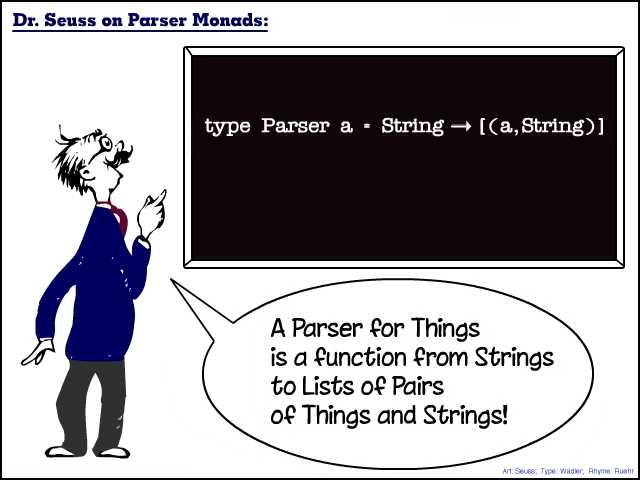
\includegraphics[scale=.4]{SeussFinal2}}\hfill\;
\end{frame}

\begin{frame}[fragile]{Modulul Parser}
{partea I}
\begin{asciihs}
  module Parser(Parser,apply,parse,char,spot,token,
    star,plus,parseInt) where

  import Char
  import Monad

  -- Tipul (incapsulat) Parser
  newtype Parser a = Parser (String -> [(a, String)])

  -- Folosirea unui parser (functie privata)
  apply :: Parser a -> String -> [(a, String)]
  apply (Parser f) s = f s

  -- Daca exista parsare, da prima varianta
  parse :: Parser a -> String -> a
  parse m s = head [ x | (x,t) <- apply m s, t == "" ]
\end{asciihs}
\end{frame}


%Module Parser

\begin{frame}[fragile]{Modulul Parser}{partea II: Parser e monadă}
\begin{asciihs}

  --   class Monad m where
  --     return :: a -> m a
  --     (>>=) :: m a -> (a -> m b) -> m b

  instance Monad Parser where
    return x  = Parser (\s -> [(x,s)])
    m >>= k   = Parser (\s ->
                   [ (y, u) |
                     (x, t) <- apply m s,
                     (y, u) <- apply (k x) t ])
\end{asciihs}
\end{frame}


%Parser is a Monad

\begin{frame}[fragile]{Modulul Parser}{partea II: Parser e monadă cu plus}
\begin{asciihs}
  --   class MonadPlus m where
  --     mzero :: m a
  --     mplus :: m a -> m a -> m a

  instance MonadPlus Parser where
    mzero      = Parser (\s -> [])
    mplus m n  = Parser (\s -> apply m s ++ apply n s)
\end{asciihs}

\begin{itemize}
\item mzero reprezintă analizorul sintactic care eșuează tot timpul
\item mplus reprezintă combinarea alternativelor
\end{itemize}

\end{frame}


%Parser is a Monad with Plus
%  -- Some monads have additional structure
%

\begin{frame}[fragile]{Parsare pentru caractere}
\begin{asciihs}
  -- Recunoasterea unui caracter
  char :: Parser Char
  char = Parser f
    where
    f []     = []
    f (c:s) = [(c,s)]

  -- Recunoasterea unui caracter cu o proprietate
  spot :: (Char -> Bool) -> Parser Char
  spot p = Parser f
    where
    f []                 = []
    f (c:s) | p c        = [(c, s)]
            | otherwise = []

  -- Recunoasterea unui anumit caracter
  token :: Char -> Parser Char
  token c = spot (== c)
\end{asciihs}
\end{frame}


%Parsing characters


\begin{frame}[fragile]{Recunoașterea unui caracter cu o proprietate}
{Gărzi și notație \lstinline$do$}
\begin{asciihs}
  spot :: (Char -> Bool) -> Parser Char
  spot p = Parser f
    where
    f []                 = []
    f (c:s) | p c        = [(c, s)]
            | otherwise = []
\end{asciihs}
e echivalentă cu
\begin{asciihs}
  spot :: (Char -> Bool) -> Parser Char
  spot p = do { c <- char; guard (p c); return c }
\end{asciihs}
\end{frame}

\begin{frame}[fragile]{Recunoașterea unui cuvânt cheie}
\begin{asciihs}
  match :: String -> Parser String
  match []      = return []
  match (x:xs) = do
                     y <- token x;
                     ys <- match xs;
                     return (y:ys)
\end{asciihs}
\end{frame}


%Parsing a string

\begin{frame}[fragile]{Recunoașterea unei secvențe repetitive}
\begin{asciihs}
  -- Steluta Kleene (zero, una sau mai multe repetitii)
  star :: Parser a -> Parser [a]
  star p = plus p `mplus` return []

  -- cel putin o repetitie
  plus :: Parser a -> Parser [a]
  plus p = do { x <- p;
                xs <- star p;
                return (x:xs) }
\end{asciihs}
\end{frame}


%Parsing a sequence

\begin{frame}[fragile]{Recunoașterea unui numar întreg}
\begin{asciihs}
  -- Recunoasterea unui numar natural
  parseNat :: Parser Int
  parseNat = do { s <- plus (spot isDigit);
                  return (read s) }

  -- Recunoasterea unui numar negativ
  parseNeg :: Parser Int
  parseNeg = do { token '-';
                  n <- parseNat
                  return (-n) }

  -- Recunoasterea unui numar intreg
  parseInt :: Parser Int
  parseInt = parseNat `mplus` parseNeg
\end{asciihs}
\end{frame}


%Parsing an integer

\begin{frame}[fragile]{Modulul Exp}
\begin{asciihs}
  module Exp where

  import Monad
  import Parser

  data Exp = Lit Int
           | Exp :+: Exp
           | Exp :*: Exp
           deriving (Eq,Show)

  evalExp   :: Exp -> Int
  evalExp   (Lit n)    = n
  evalExp   (e :+: f) = evalExp e + evalExp f
  evalExp   (e :*: f) = evalExp e * evalExp f
\end{asciihs}
\end{frame}


%Module Exp


\begin{frame}[fragile]{Recunoașterea unei expresii}
\begin{asciihs}
  parseExp :: Parser Exp
  parseExp = parseLit `mplus` parseAdd `mplus` parseMul
    where
    parseLit = do { n <- parseInt;
                    return (Lit n) }
    parseAdd = do { token '(';
                    d <- parseExp;
                    token '+';
                    e <- parseExp;
                    token ')';
                    return (d :+: e) }
    parseMul = do { token '(';
                    d <- parseExp;
                    token '*';
                    e <- parseExp;
                    token ')';
                    return (d :*: e) }
\end{asciihs}
\end{frame}


%Parsing an expression

\begin{frame}[fragile]{Recunoașterea unei expresii}{Test}
\begin{asciihs}
  *Exp> parse parseExp "(1+(2*3))"
  Lit 1 :+: (Lit 2 :*: Lit 3)
  *Exp> evalExp (parse parseExp "(1+(2*3))")
  7
  *Exp> parse parseExp "((1+2)*3)"
  (Lit 1 :+: Lit 2) :*: Lit 3
  *Exp> evalExp (parse parseExp "((1+2)*3)")
  9
\end{asciihs}
\end{frame}



\section{Evaluare cu efecte laterale}

\subsection{Sintaxă abstractă}

\begin{frame}[fragile]{Lambda calcul cu întregi}
{Sintaxă}
\begin{asciihs}
type Name = String
data Term
  = Var Name
  | Con Int
  | Add Term Term
  | Lam Name Term
  | App Term Term
\end{asciihs}
\end{frame}


\begin{frame}[fragile]
{Valori și medii de evaluare}
\begin{asciihs}
data Value m
  = Wrong
  | Num Int
  | Fun (Value m -> m (Value m))
  
instance Show (Value m) where
  show Wrong = "<wrong>"
  show (Num i) = show i
  show (Fun f) = "<function>"
\end{asciihs}
\end{frame}

\begin{frame}[fragile]
{Mediul de variabile}
\begin{asciihs}
type Environment m = [(Name,Value m)]

lookUp :: Monad m => Name -> Environment m -> m (Value m)
lookUp _ [] 
  = return Wrong
lookUp x ((y,b):e)
  = if x == y then return b else lookUp x e
\end{asciihs}
\end{frame}

\begin{frame}[fragile]
{Evaluare}{Variabile și valori}
\begin{asciihs}
interp :: Monad m => Term -> Environment m -> m (Value m)
interp (Var x) e   = lookUp x e
interp (Con i) e   = return (Num i)
interp (Lam x v) e = return (Fun (\a -> interp v ((x,a):e)))
\end{asciihs}
\end{frame}



\begin{frame}[fragile]
{Evaluare}{Adunare}
\begin{asciihs}
interp (Add u v) e = 
  do {
    a <- interp u e;
    b <- interp v e;
    add a b
  }

add :: (Monad m) => Value m -> Value m -> m (Value m)
add (Num i) (Num j) = return (Num (i+j))
add _       _       = return Wrong
\end{asciihs}
\end{frame}

\begin{frame}[fragile]
{Evaluare}{Aplicarea funcțiilor}
\begin{asciihs}
interp (App t u) e = 
  do {
    f <- interp t e;
    a <- interp u e;
    apply f a
  }


apply :: (Monad m) => Value m -> Value m -> m (Value m)
apply (Fun k) a = k a
apply _ _ = return Wrong
\end{asciihs}
\end{frame}


\begin{frame}[fragile]{Interpretare în monada Identitate}
\begin{asciihs}
newtype Identity a = Id a
instance Monad Identity where
  return a   = Id a
  Id a >>= k = k a

instance (Show a) => Show (Identity a) where
  show (Id a) = show a

evalId :: Term -> String
evalId t = show ( interp t ([]::Environment Identity) )
\end{asciihs}
\begin{itemize}
\item Obținem interpretorul standard discutat în cursurile trecute
\end{itemize}
\end{frame}


\begin{frame}[fragile]{Interpretare în monada Eroare}
\begin{asciihs}
data Error a = Success a | Error String
  (deriving Show)

instance Monad Error where
  return a = Success a
  fail   s = Error s
  (Success a) >>= k = k a
  (Error s)   >>= k = Error s
  
  
lookUp x [] = fail ("Unbound variable " ++ x)
add a b   = fail ("Should be numbers: " ++ show a ++ 
                                    "," ++ show b)
add f _   = fail ("Should be function: " ++ show f)
\end{asciihs}
\end{frame}

%\begin{frame}[fragile]{Interpretare în monada Stare}
%\begin{asciihs}
%data MState state a = MState (state -> (a,state))
%\end{asciihs}
%\end{frame}

\end{document}



